\section{Les catégories: premier contact}
L'intérêt de se tourner vers la théorie des catégories est de guider le
design de la bibliothèque pour obtenir des interfaces très généraux et
spécifiés clairement, formellement. La généralité de la théorie permet
d'avoir des interfaces qui sont très abstraits et qui en couvrent donc
très large, ce qui réduit la complexité globale de la bibliothèque. La
capacité de formaliser ces interfaces permet d'automatiser une bonne partie
des tests et de raisonner à propos des programmes écrits avec Hana de manière
très précise, quasiment mathématique.

\begin{définition}[Catégorie]
    Une catégorie $\C$ est composée de trois choses:
    \begin{enumerate}
        \item Une collection d'objets, habituellement notée $\ob(\C)$.
        \item Une collection de flèches (aussi appelées morphismes) entre ces
              objets, habituellement notée $\hom(\C)$.
        \item Une opération binaire, habituellement notée $\circ$, permettant de
              composer n'importe quelle paire de flèches dont les sources et
              destinations sont compatibles pour en obtenir une troisième.
    \end{enumerate}
\end{définition}

Pour que $\C$ soit une catégorie, ces ``choses'' doivent aussi respecter
certaines propriétés, qui seront expliquées un peu plus bas. Avant de
continuer, il est important de préciser quelques détails et d'introduire
un peu de notation qui rendra notre tâche plus facile pour la suite. D'abord,
pour deux objets $X, Y \in \ob(\C)$, on note la collection des flèches allant
de $X$ vers $Y$ par $\hom(X, Y)$, ou encore $\hom_\C(X, Y)$ lorsque la catégorie
$\C$ n'est pas évidente à partir du contexte. On utilise aussi la notation
$f : X \to Y$ pour dire que $f$ est une flèche allant de $X$ vers $Y$,
c'est-à-dire que $f \in \hom(X, Y)$. On dit alors que $f$ est de source
$X$ et de destination $Y$, noté $\dom(f)$ et $\range(f)$ respectivement.

Ensuite, il est important de bien comprendre qu'on ne parle pas en réalité
d'une seule opération binaire, mais bien d'une opération binaire pour chaque
triplet d'objets $X, Y, Z \in \ob(\C)$. En effet, on souhaite définir notre
opération binaire de manière à ce qu'elle puisse composer n'importe quelles
deux flèches dont les sources et destinations sont compatibles, c'est-à-dire
que pour des flèches $f : Y \to Z$ et $g : X \to Y$, on puisse écrire
$f \circ g$. La définition de $\circ$ doit donc être de la forme
\begin{align*}
    \circ : \hom(Y, Z) \times \hom(X, Y) &\to \hom(X, Z) \\
             f, g &\mapsto f \circ g
\end{align*}

Il est donc nécessaire de parler d'une telle opération $\circ$ pour chaque
paire de $\hom$-classe $\left(\hom(Y, Z), \hom(X, Y)\right)$, ou, de manière
équivalente, pour chaque triplet d'objets $\left(X, Y, Z\right)$. Pour justifier
rigoureusement notre abus de langage, appelons $\circ_{\left(X,Y,Z\right)}$
l'opération binaire associée au triplet d'objets $\left(X,Y,Z\right)$.
Il suffit maintenant de définir la composition comme
\begin{align*}
    \circ : \bigcup \left\{ \dom(\circ_{\left(X,Y,Z\right)})
                            \suchthat X, Y, Z \in \ob(\C) \right\} &\to \hom(\C) \\
           f, g &\mapsto f \circ_{\left(\dom(g), \range(g), \range(f)\right)} g
\end{align*}
, ce qui nous permet de composer n'importe quelles deux flèches dont les sources
et destinations sont compatibles sans s'enfarger dans les fleurs du tapis. Nous
sommes maintenant prêts à passer aux propriétés qui doivent être satisfaites
pour qu'on ait bien une catégorie. D'abord, pour tout objet $X \in \ob(\C)$,
il doit exister une flèche de $X$ vers lui-même, qu'on appelle généralement
identité (sur $X$):
\[
    \id_X : X \to X
\]

Ensuite, la composition $\circ$ définie plus haut doit être associative,
c'est-à-dire que pour toutes flèches $f : C \to D$, $g : B \to C$ et
$h : A \to B$, on doit avoir
\[
    (f \circ g) \circ h = f \circ (g \circ h)
\]

Finalement, on doit avoir que les identités sont des éléments neutres de la
composition, c'est-à-dire que pour toute flèche $f : A \to B$,
\[
    f = \id_B \circ f = f \circ \id_A
\]

Il est intéressant d'observer que ces deux dernières propriétés sont
semblables à demander que $\left(\hom(\C), \circ\right)$ soit un monoïde.
Ce n'est évidemment pas le cas puisqu'on a plusieurs identités et parce
que $\circ$ n'est pas définie sur la totalité de $\hom(\C) \times \hom(\C)$,
mais l'intuition reste utile.


%%%%%%%%%%%%%%%%%%%%%%%%%%%%%%%%%%%%%%%%%%%%%%%%%%%%%%%%%%%%%%%%%%%%%%%%%%%%%%
\subsection{Exemples de catégories}
Avec la définition d'une catégorie qui vient d'être faite, il est un peu
difficile de voir comment les catégories peuvent se matérialiser. Nous
explorerons donc maintenant des catégories simples qui permettent de se
forger une intuition dans le but éventuel d'étudier des catégories plus utiles.
Dans cet optique, on se doit de commencer par la catégorie la plus simple;
la catégorie vide. Comme son nom l'indique, cette catégorie n'a pas d'objets
ni de flèches, et sa loi de composition est une application vide
$\circ : \emptyset \times \emptyset \to \emptyset$. Les propriétés d'une
catégorie sont trivialement satisfaites. Une autre catégorie simple (et
peu utile) est la catégorie triviale, qui ne contient qu'un seul objet
et sa flèche identité:

\centerline{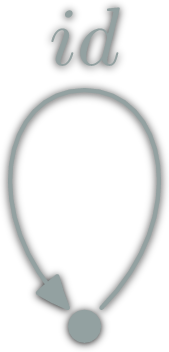
\includegraphics[scale=0.3]{figures/trivial}}

De manière générale, on peut voir une catégorie comme un graphe dirigé avec
certaines propriétés. Par exemple, le graphe suivant est une catégorie:

% TODO
\centerline{\tikz \draw (0,0) rectangle (3, 2);}

Les objets sont les sommets du graphe, les flèches sont les arrêtes et la loi
de composition est une application qui associe à deux arrêtes $u$ et $v$ un
troisième sommet qui part de la source de $u$ jusqu'à la destination de $v$.
Bien entendu, tous les graphes ne sont pas des catégories. Par exemple, le
graphe suivant ne peut pas être une catégorie:

% TODO
\centerline{\tikz \draw (0,0) rectangle (3, 2);}

En effet, il n'y a pas d'arrête qui part du sommet $a$ vers lui-même, ce qui
ne respecte pas le fait que chaque objet doit avoir une flèche identité. Aussi,
bien qu'il respecte les identités, le graphe suivant ne peut pas être une
catégorie:

% TODO
\centerline{\tikz \draw (0,0) rectangle (3, 2);}

En effet, il existe une arrête entre les sommets $a$ et $b$ et une arrête
entre les sommets $b$ et $c$, mais il n'y en a pas entre les sommets $a$ et
$c$. Si on essayait de définir la loi de composition, on se rendrait compte
qu'il n'y a pas de valeur possible pour $u \circ v$. Ainsi, la composition
serait mal définie et le graphe ne peut pas représenter une catégorie. En
général, on peut créer une catégorie à partir de n'importe quel graphe dirigé
en ajoutant simplement les flèches manquantes.

Une des raisons d'étudier les catégories est leur capacité d'unifier des
notions sous un même emblème. Suivant cette ligne de pensée, il est possible
d'inscrire la plupart des structures provenant de l'algèbre abstraite dans
un contexte catégorique. On commence d'abord par la catégorie $\mathrm{Set}$,
dont les objets sont les ensembles, les flèches sont les applications
ensemblistes et la composition est la composition usuelle de fonctions.
On peut ensuite ajouter de la structure à ces ensembles et demander que
les applications ensemblistes respectent cette structure. Ceci nous mène
à considérer, par exemple, la catégorie $\mathrm{Grp}$, où les objets sont
les groupes et les flèches sont des homomorphismes de groupe, avec la
composition usuelle. On peut continuer sur ce chemin et considérer la
catégorie $\mathrm{Ring}$ des anneaux, où les flèches sont des homomorphismes
d'anneaux, puis la catégorie $\mathrm{K-Vect}$ des espaces vectoriels sur un
corps $K$, où les flèches sont les transformations K-linéaires, et ainsi de
suite. Du côté de l'analyse, on peut considérer par exemple la catégorie
$\mathrm{Met}$ des espaces métriques, où les flèches sont les applications
1-Lipschitz. Les exemples sont nombreux; en fait, la plupart des théories
mathématiques peuvent être exprimés dans ce cadre, parfois moyennant une
petite dose d'imagination.


%%%%%%%%%%%%%%%%%%%%%%%%%%%%%%%%%%%%%%%%%%%%%%%%%%%%%%%%%%%%%%%%%%%%%%%%%%%%%%
\subsection{La catégorie Hana}
La catégorie Hana est définie de manière similaire à Hask, mais les types
sont remplacés par la notion plus générale de type généralisé présentée
précédemment. En particulier, les objets de Hana sont les types généralisés:
\[
    \ob(Hana) := \{ T \suchthat \text{T est un type généralisé} \}
\]

Les flèches de Hana sont les fonctions génériques qui travaillent sur des
objets ayant un certain type généralisé, et ce peu importe le type réel de ces
objets. Plus précisément, soit $X, Y \in \ob(Hana)$, c'est-à-dire que $X$ et $Y$
sont deux types généralisés. Une flèche $f : X \to Y$ est un objet C++, disons
\icpp{f}, avec un \icpp{operator()} tel que $\forall x \in X$,
\begin{enumerate}
    \item l'expression \icpp{f(x)} est bien formée, c'est-à-dire qu'elle compile
    \item ${\tt f(x)} \in Y$, c'est-à-dire que le type généralisé de l'expression \icpp{f(x)} est $Y$
    \item l'expression \icpp{f(x)} n'a pas d'effets de bord
\end{enumerate}

La propriété (3) est nécessaire pour s'assurer que les fonctions qu'on
considère sont des fonctions au sens mathématique, c'est-à-dire que
\[
    x = y \implies f(x) = f(y)
\]

Sans se restreindre explicitement à cette classe de fonctions, on perdrait la
capacité de raisonner mathématiquement à propos des fonctions de Hana puisque
le langage C++ n'est pas pur, contrairement au Haskell. Ce n'est cependant pas
une restriction qui nous handicap beaucoup, puisque Hana s'intéresse surtout à
la manipulation d'objets hétérogènes, ce qui requiert l'utilisation d'un style
de programmation fonctionnel de toute façon.

Finalement, la loi de composition sur Hana est, sans grande surprise,
l'extension de la composition de fonctions usuelle aux fonctions
\textit{templates} qui constituent les flèches de Hana, $\hom(Hana)$.
Rigoureusement, soit $X, Y, Z \in \ob(Hana)$, c'est-à-dire que $X$, $Y$ et
$Z$ sont des types généralisés. On peut définir la composition par
\begin{cpp}
    template <typename X, typename Y, typename Z>
    auto compose = [](auto f, auto g) {
        return [=](auto x) {
            static_assert(std::is_same<datatype_t<decltype(x)>, X>{}, "");
            static_assert(std::is_same<datatype_t<decltype(g(x))>, Y>{}, "");
            static_assert(std::is_same<datatype_t<decltype(f(g(x)))>, Z>{}, "");
            return f(g(x));
        };
    };
\end{cpp}

Ainsi, \icpp{compose<X, Y, Z>} peut être appelée avec n'importe quelle fonctions
$f$ et $g$, mais celles dont les domaines et codomaines ne coïncident pas
avec \icpp{X}, \icpp{Y} et \icpp{Z} résulteront en une erreur de compilation.
Dans la réalité, il est trop répétitif de préciser les types $X$, $Y$ et $Z$
et on préfère la définition suivante pour \icpp{compose}:
\begin{cpp}
    auto compose = [](auto f, auto g) {
        return [=](auto x) {
            return f(g(x));
        };
    };
\end{cpp}

La tâche de s'assurer que les domaines et codomaines sont respectés est ainsi
laissée au programmeur, mais l'interface qui en résulte est beaucoup plus
facile à utiliser. Dans les preuves, la première définition de \icpp{compose}
sera généralement utilisée, pour mettre en évidence les types généralisés des
fonctions qui sont composées.

Il nous reste à démontrer que Hana est bien une catégorie. Pour ce faire,
il suffit de vérifier qu'il existe une flèche identité pour chaque objet de
la catégorie et que la composition est bien associative. D'abord, la flèche
identité d'un type généralisé peut être définie en utilisant une fonction
\textit{template} ou une fonction anonyme générique de la manière suivante:
\begin{cpp}
    template <typename X>
    auto id = [](auto x) {
        static_assert(std::is_same<datatype_t<decltype(x), X>>{}, "");
        return x;
    };
\end{cpp}

Ainsi, étant donné un type généralisé \icpp{X}, l'identité sur \icpp{X} est
\icpp{id<X>}. Puisque le type C++ de l'argument de \icpp{id<X>} est quelconque,
on peut passer n'importe quel objet à cette fonction, tant que le type
généralisé de cet objet est exactement \icpp{X}. Si ce n'est pas le cas,
le compilateur rapportera une erreur de compilation. De plus, il est clair
que l'identité est un élément neutre de la loi de composition. En effet, soit
$A$ et $B$ des types généralisés et $f : A \to B$ une fonction. Alors,
\begin{cpp}
    compose<A, B, B>(id<B>, f) == [](auto x) { return id<B>(f(x)); }
                               == [](auto x) { return f(x); }
                               == f
\end{cpp}

De manière similaire,
\begin{cpp}
    compose<A, A, B>(f, id<A>) == [](auto x) { return f(id<A>(x)); }
                               == [](auto x) { return f(x); }
                               == f
\end{cpp}

ce qui montre que l'identité est bien l'élément neutre de la composition.
Ensuite, il reste à montrer que la composition est associative, ce qui n'est
pas difficile non plus. Pour des types généralisés $A, B, C, D$, soit
$f : A \to B$, $g : B \to C$ et $h : C \to D$ des fonctions. Alors,
\begin{cpp}
    compose<A, C, D>(h, compose<A, B, C>(g, f))
        == [](auto x) { return h(compose<A, B, C>(g, f)(x)); }
        == [](auto x) { return h([](auto x) { return g(f(x)); }(x)); }
        == [](auto x) { return h(g(f(x))); }
\end{cpp}

De l'autre côté, on obtient que
\begin{cpp}
    compose<A, B, D>(compose<B, C, D>(h, g), f)
        == [](auto x) { return compose<B, C, D>(h, g)(f(x)); }
        == [](auto x) { return [](auto x) { return h(g(x)); }(f(x)); }
        == [](auto x) { return h(g(f(x))); }
\end{cpp}

ce qui montre que la composition est associative, et Hana est donc bien une
catégorie.
